\documentclass[14pt]{extbook}
\usepackage{multicol, enumerate, enumitem, hyperref, color, soul, setspace, parskip, fancyhdr} %General Packages
\usepackage{amssymb, amsthm, amsmath, latexsym, units, mathtools} %Math Packages
\everymath{\displaystyle} %All math in Display Style
% Packages with additional options
\usepackage[headsep=0.5cm,headheight=12pt, left=1 in,right= 1 in,top= 1 in,bottom= 1 in]{geometry}
\usepackage[usenames,dvipsnames]{xcolor}
\usepackage{dashrule}  % Package to use the command below to create lines between items
\newcommand{\litem}[1]{\item#1\hspace*{-1cm}\rule{\textwidth}{0.4pt}}
\pagestyle{fancy}
\lhead{Progress Quiz 6}
\chead{}
\rhead{Version A}
\lfoot{9689-6866}
\cfoot{}
\rfoot{Spring 2021}
\begin{document}

\begin{enumerate}
\litem{
Write the equation of the line in the graph below in Standard form $Ax+By=C$. Then, choose the intervals that contain $A, B, \text{ and } C$.
\begin{center}
    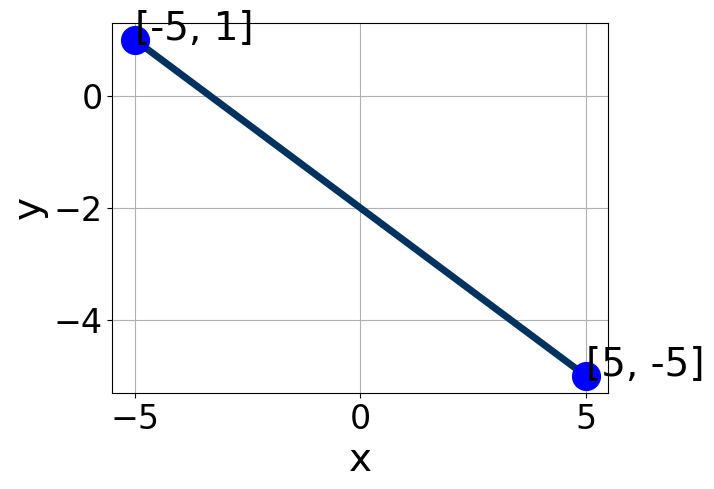
\includegraphics[width=0.5\textwidth]{../Figures/linearGraphToStandardA.png}
\end{center}
\begin{enumerate}[label=\Alph*.]
\item \( A \in [-0.67, 0.33], \hspace{3mm} B \in [-2.52, -0.91], \text{ and } \hspace{3mm} C \in [-5.6, 0.9] \)
\item \( A \in [-0.67, 0.33], \hspace{3mm} B \in [0.93, 2.65], \text{ and } \hspace{3mm} C \in [-0.4, 3.2] \)
\item \( A \in [-3, -1], \hspace{3mm} B \in [1.84, 3.16], \text{ and } \hspace{3mm} C \in [4.5, 9.8] \)
\item \( A \in [0, 3], \hspace{3mm} B \in [-3.7, -2.3], \text{ and } \hspace{3mm} C \in [-6.3, -5.4] \)
\item \( A \in [0, 3], \hspace{3mm} B \in [1.84, 3.16], \text{ and } \hspace{3mm} C \in [4.5, 9.8] \)

\end{enumerate} }
\litem{
Find the equation of the line described below. Write the linear equation as $ y=mx+b $ and choose the intervals that contain $m$ and $b$.\[ \text{Perpendicular to } 3 x + 4 y = 15 \text{ and passing through the point } (3, -2). \]\begin{enumerate}[label=\Alph*.]
\item \( m \in [1.14, 1.87] \hspace*{3mm} b \in [-6.48, -5.18] \)
\item \( m \in [-1.93, -0.96] \hspace*{3mm} b \in [1.1, 2.43] \)
\item \( m \in [1.14, 1.87] \hspace*{3mm} b \in [-5.47, -4.87] \)
\item \( m \in [1.14, 1.87] \hspace*{3mm} b \in [5.11, 7.08] \)
\item \( m \in [0.61, 1.11] \hspace*{3mm} b \in [-6.48, -5.18] \)

\end{enumerate} }
\litem{
First, find the equation of the line containing the two points below. Then, write the equation as $ y=mx+b $ and choose the intervals that contain $m$ and $b$.\[ (11, 2) \text{ and } (6, 6) \]\begin{enumerate}[label=\Alph*.]
\item \( m \in [-1.06, 0.03] \hspace*{3mm} b \in [-10.85, -10.16] \)
\item \( m \in [-1.06, 0.03] \hspace*{3mm} b \in [-9.81, -8.91] \)
\item \( m \in [-1.06, 0.03] \hspace*{3mm} b \in [10.19, 11.58] \)
\item \( m \in [0.65, 1.18] \hspace*{3mm} b \in [0.83, 1.78] \)
\item \( m \in [-1.06, 0.03] \hspace*{3mm} b \in [-1.99, 0.9] \)

\end{enumerate} }
\litem{
Write the equation of the line in the graph below in Standard form $Ax+By=C$. Then, choose the intervals that contain $A, B, \text{ and } C$.
\begin{center}
    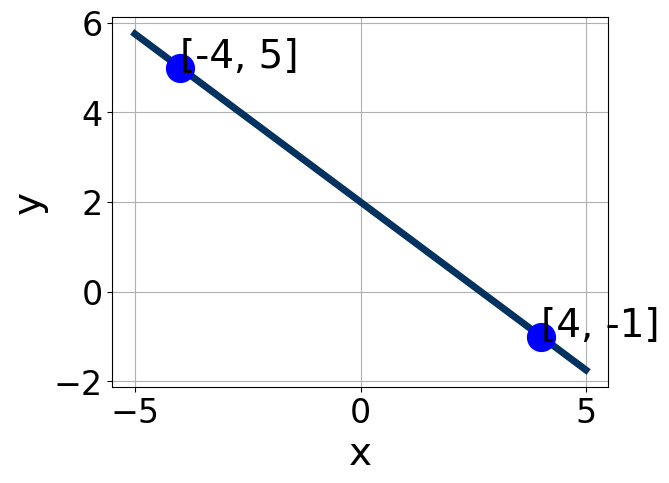
\includegraphics[width=0.5\textwidth]{../Figures/linearGraphToStandardCopyA.png}
\end{center}
\begin{enumerate}[label=\Alph*.]
\item \( A \in [-0.69, 0.72], \hspace{3mm} B \in [-0.02, 1.44], \text{ and } \hspace{3mm} C \in [-1.1, -0.4] \)
\item \( A \in [1.1, 3.35], \hspace{3mm} B \in [-3.02, -1.02], \text{ and } \hspace{3mm} C \in [1.7, 5] \)
\item \( A \in [-3.76, -1.16], \hspace{3mm} B \in [-3.02, -1.02], \text{ and } \hspace{3mm} C \in [1.7, 5] \)
\item \( A \in [-0.69, 0.72], \hspace{3mm} B \in [-1.53, -0.5], \text{ and } \hspace{3mm} C \in [0.7, 2.2] \)
\item \( A \in [1.1, 3.35], \hspace{3mm} B \in [2.82, 3.42], \text{ and } \hspace{3mm} C \in [-5.3, -2.6] \)

\end{enumerate} }
\litem{
Solve the equation below. Then, choose the interval that contains the solution.\[ -5(-10x + 12) = -8(-4x + 2) \]\begin{enumerate}[label=\Alph*.]
\item \( x \in [0.4, 1.4] \)
\item \( x \in [2.1, 3.1] \)
\item \( x \in [4, 5.2] \)
\item \( x \in [-4.8, -3.6] \)
\item \( \text{There are no real solutions.} \)

\end{enumerate} }
\litem{
Solve the linear equation below. Then, choose the interval that contains the solution.\[ \frac{-6x -6}{5} - \frac{-3x + 4}{2} = \frac{5x + 3}{6} \]\begin{enumerate}[label=\Alph*.]
\item \( x \in [-2.9, -0.1] \)
\item \( x \in [0.2, 1] \)
\item \( x \in [-26.4, -20.7] \)
\item \( x \in [-8, -5.6] \)
\item \( \text{There are no real solutions.} \)

\end{enumerate} }
\litem{
First, find the equation of the line containing the two points below. Then, write the equation as $ y=mx+b $ and choose the intervals that contain $m$ and $b$.\[ (-11, 4) \text{ and } (5, -9) \]\begin{enumerate}[label=\Alph*.]
\item \( m \in [-1, 0] \hspace*{3mm} b \in [-14.9, -13.7] \)
\item \( m \in [0.5, 2] \hspace*{3mm} b \in [-13.8, -11.7] \)
\item \( m \in [-1, 0] \hspace*{3mm} b \in [-6.8, -1] \)
\item \( m \in [-1, 0] \hspace*{3mm} b \in [10.8, 16.5] \)
\item \( m \in [-1, 0] \hspace*{3mm} b \in [3.3, 6.9] \)

\end{enumerate} }
\litem{
Find the equation of the line described below. Write the linear equation as $ y=mx+b $ and choose the intervals that contain $m$ and $b$.\[ \text{Perpendicular to } 5 x + 4 y = 10 \text{ and passing through the point } (-10, 10). \]\begin{enumerate}[label=\Alph*.]
\item \( m \in [0.25, 1.24] \hspace*{3mm} b \in [-20.5, -16.7] \)
\item \( m \in [-1.57, 0.33] \hspace*{3mm} b \in [0.3, 2.1] \)
\item \( m \in [0.25, 1.24] \hspace*{3mm} b \in [14.6, 19] \)
\item \( m \in [0.25, 1.24] \hspace*{3mm} b \in [18.4, 20.2] \)
\item \( m \in [0.93, 1.35] \hspace*{3mm} b \in [14.6, 19] \)

\end{enumerate} }
\litem{
Solve the linear equation below. Then, choose the interval that contains the solution.\[ \frac{-8x + 7}{7} - \frac{5x -7}{3} = \frac{-7x + 5}{4} \]\begin{enumerate}[label=\Alph*.]
\item \( x \in [0.1, 0.9] \)
\item \( x \in [1.8, 2.9] \)
\item \( x \in [8.1, 8.6] \)
\item \( x \in [-2.8, -1.7] \)
\item \( \text{There are no real solutions.} \)

\end{enumerate} }
\litem{
Solve the equation below. Then, choose the interval that contains the solution.\[ -12(17x + 5) = -4(-19x + 10) \]\begin{enumerate}[label=\Alph*.]
\item \( x \in [-0.08, 0.19] \)
\item \( x \in [-0.51, -0.33] \)
\item \( x \in [0.13, 0.7] \)
\item \( x \in [-1.06, -0.64] \)
\item \( \text{There are no real solutions.} \)

\end{enumerate} }
\end{enumerate}

\end{document}